% Readable scenario-specific provenance projection — SUPPORT2 180-day
% mortality (scenario 000008). This is an editorial readability adaptation
% of the canonical provenance.provn for that scenario run, not prov_to_dot
% output; the complete original Graphviz/PROV artifacts remain published per
% scenario (see
% coinfosim-report-latex/figures/provenance/provenance_support2_000008.pdf
% and the scenario's semantic_manifest.json / provenance.{provjson,provn,ttl}).
% Node/relation types follow docs/semantics/provenance_mapping.md exactly,
% including RandomForestCalibrationArtifact (coinfosim:RandomForestCalibrationArtifact),
% confirmed `used` by all three simulation-run activities in provenance.provn.
% PreparedDataset is omitted here (kept only in the generic diagram) to leave
% room for the dataset-specific notes below. The dashed grey notes attach
% dataset-specific facts (target construction, excluded predictors, cohort,
% stratified split) documented in
% coinfosim-report-latex/chapters/04_datasets.tex (Section on SUPPORT2) —
% they are captions, not additional PROV nodes. This diagram does not imply
% clinical validation. ArtifactRecovery/RecoveredArtifactSet/CodeRevision are
% omitted for the same reason as in the generic diagram: report-regeneration
% metadata, not experimental science provenance. Compilation: xelatex.
\documentclass[tikz,border=6pt]{standalone}
% Shared visual grammar for CoInfoSim's readable TikZ provenance diagrams.
% Included by the generic model and by the three scenario-specific
% projections (Occupancy, Air Quality, SUPPORT2) so that node color/shape and
% relation-arrow style are identical across the whole diagram family:
%   prov:Entity        -> yellow, rounded-corner box
%   prov:Activity       -> blue, sharp-corner box
%   prov:SoftwareAgent   -> orange, sharp-corner box (rounder pill)
%   used / wasGeneratedBy / wasDerivedFrom / wasAssociatedWith -> one arrow
%   family per relation, labeled in italics along the edge.
% These diagrams are editorial/readability projections of the canonical
% prov.model.ProvDocument; they are not prov_to_dot output. See
% docs/semantics/provenance_mapping.md for the authoritative role table.
% Preâmbulo compartilhado dos diagramas conceituais do relatório CoInfoSim.
% Compilação: xelatex (determinística; nenhum dado experimental é usado).
\usepackage{fontspec}
\setmainfont{Liberation Sans}
\setsansfont{Liberation Sans}
\usepackage{amsmath}
\usepackage{bm}
\usepackage{tikz}
\usetikzlibrary{arrows.meta,positioning,calc,fit,backgrounds,decorations.pathreplacing,matrix,patterns}
\definecolor{CoinAccent}{RGB}{25,80,140}
\definecolor{CoinAccentDark}{RGB}{18,55,95}
\definecolor{CoinAccentPale}{RGB}{237,242,248}
\definecolor{CoinGray}{RGB}{95,95,95}
\definecolor{CoinGrayPale}{RGB}{246,246,246}
\definecolor{CoinWin}{RGB}{76,140,90}    % verde discreto (vitória)
\definecolor{CoinLose}{RGB}{182,88,79}   % vermelho discreto (derrota)
\tikzset{
  bloco/.style={draw=CoinAccentDark, fill=CoinAccentPale, rounded corners=1.2pt,
                align=center, font=\small, inner sep=4pt, minimum height=7mm},
  bloconeutro/.style={draw=CoinGray, fill=CoinGrayPale, rounded corners=1.2pt,
                align=center, font=\small, inner sep=4pt, minimum height=7mm},
  blocoreal/.style={draw=CoinAccentDark, fill=white, rounded corners=1.2pt,
                align=center, font=\small, inner sep=4pt, minimum height=7mm},
  seta/.style={-{Stealth[length=2.4mm]}, thick, CoinAccentDark},
  setacinza/.style={-{Stealth[length=2.4mm]}, thick, CoinGray},
  rotulo/.style={font=\footnotesize\itshape, text=CoinGray, align=center},
}


\definecolor{ProvEntity}{RGB}{250,232,168}
\definecolor{ProvEntityBorder}{RGB}{176,141,42}
\definecolor{ProvActivity}{RGB}{188,206,235}
\definecolor{ProvActivityBorder}{RGB}{47,86,145}
\definecolor{ProvAgent}{RGB}{248,196,120}
\definecolor{ProvAgentBorder}{RGB}{191,120,20}
\definecolor{ProvNote}{RGB}{255,255,255}
\definecolor{ProvNoteBorder}{RGB}{170,170,170}

\tikzset{
  entidade/.style={draw=ProvEntityBorder, fill=ProvEntity, rounded corners=6pt,
                align=center, font=\scriptsize, inner sep=4pt, minimum height=8.5mm, minimum width=3.65cm},
  atividade/.style={draw=ProvActivityBorder, fill=ProvActivity, rounded corners=1pt,
                align=center, font=\scriptsize, inner sep=4pt, minimum height=8.5mm, minimum width=3.65cm},
  agente/.style={draw=ProvAgentBorder, fill=ProvAgent, rounded corners=1pt,
                align=center, font=\scriptsize, inner sep=4pt, minimum height=8mm, minimum width=3.0cm},
  nota/.style={draw=ProvNoteBorder, fill=ProvNote, rounded corners=2pt, dashed,
                align=left, font=\fontsize{6.2}{7.4}\selectfont, text=CoinGray,
                inner sep=3pt},
  % Relation families: one arrow style per PROV relation, reused identically
  % across every diagram in the family.
  usedrel/.style={-{Stealth[length=2.0mm]}, thick, CoinGray},
  usedrelfina/.style={-{Stealth[length=1.8mm]}, thin, CoinGray},
  generatedrel/.style={-{Stealth[length=2.0mm]}, thick, CoinGray},
  derivedrel/.style={-{Stealth[length=1.8mm]}, thick, dashed, ProvAgentBorder},
  associatedrel/.style={-{Stealth[length=1.6mm]}, thin, dash dot, ProvAgentBorder},
  rlabel/.style={font=\tiny\itshape, text=CoinGray, fill=white, inner sep=1pt},
}

\tikzset{relacao/.style={usedrel}, relacaofina/.style={usedrelfina}}

\begin{document}
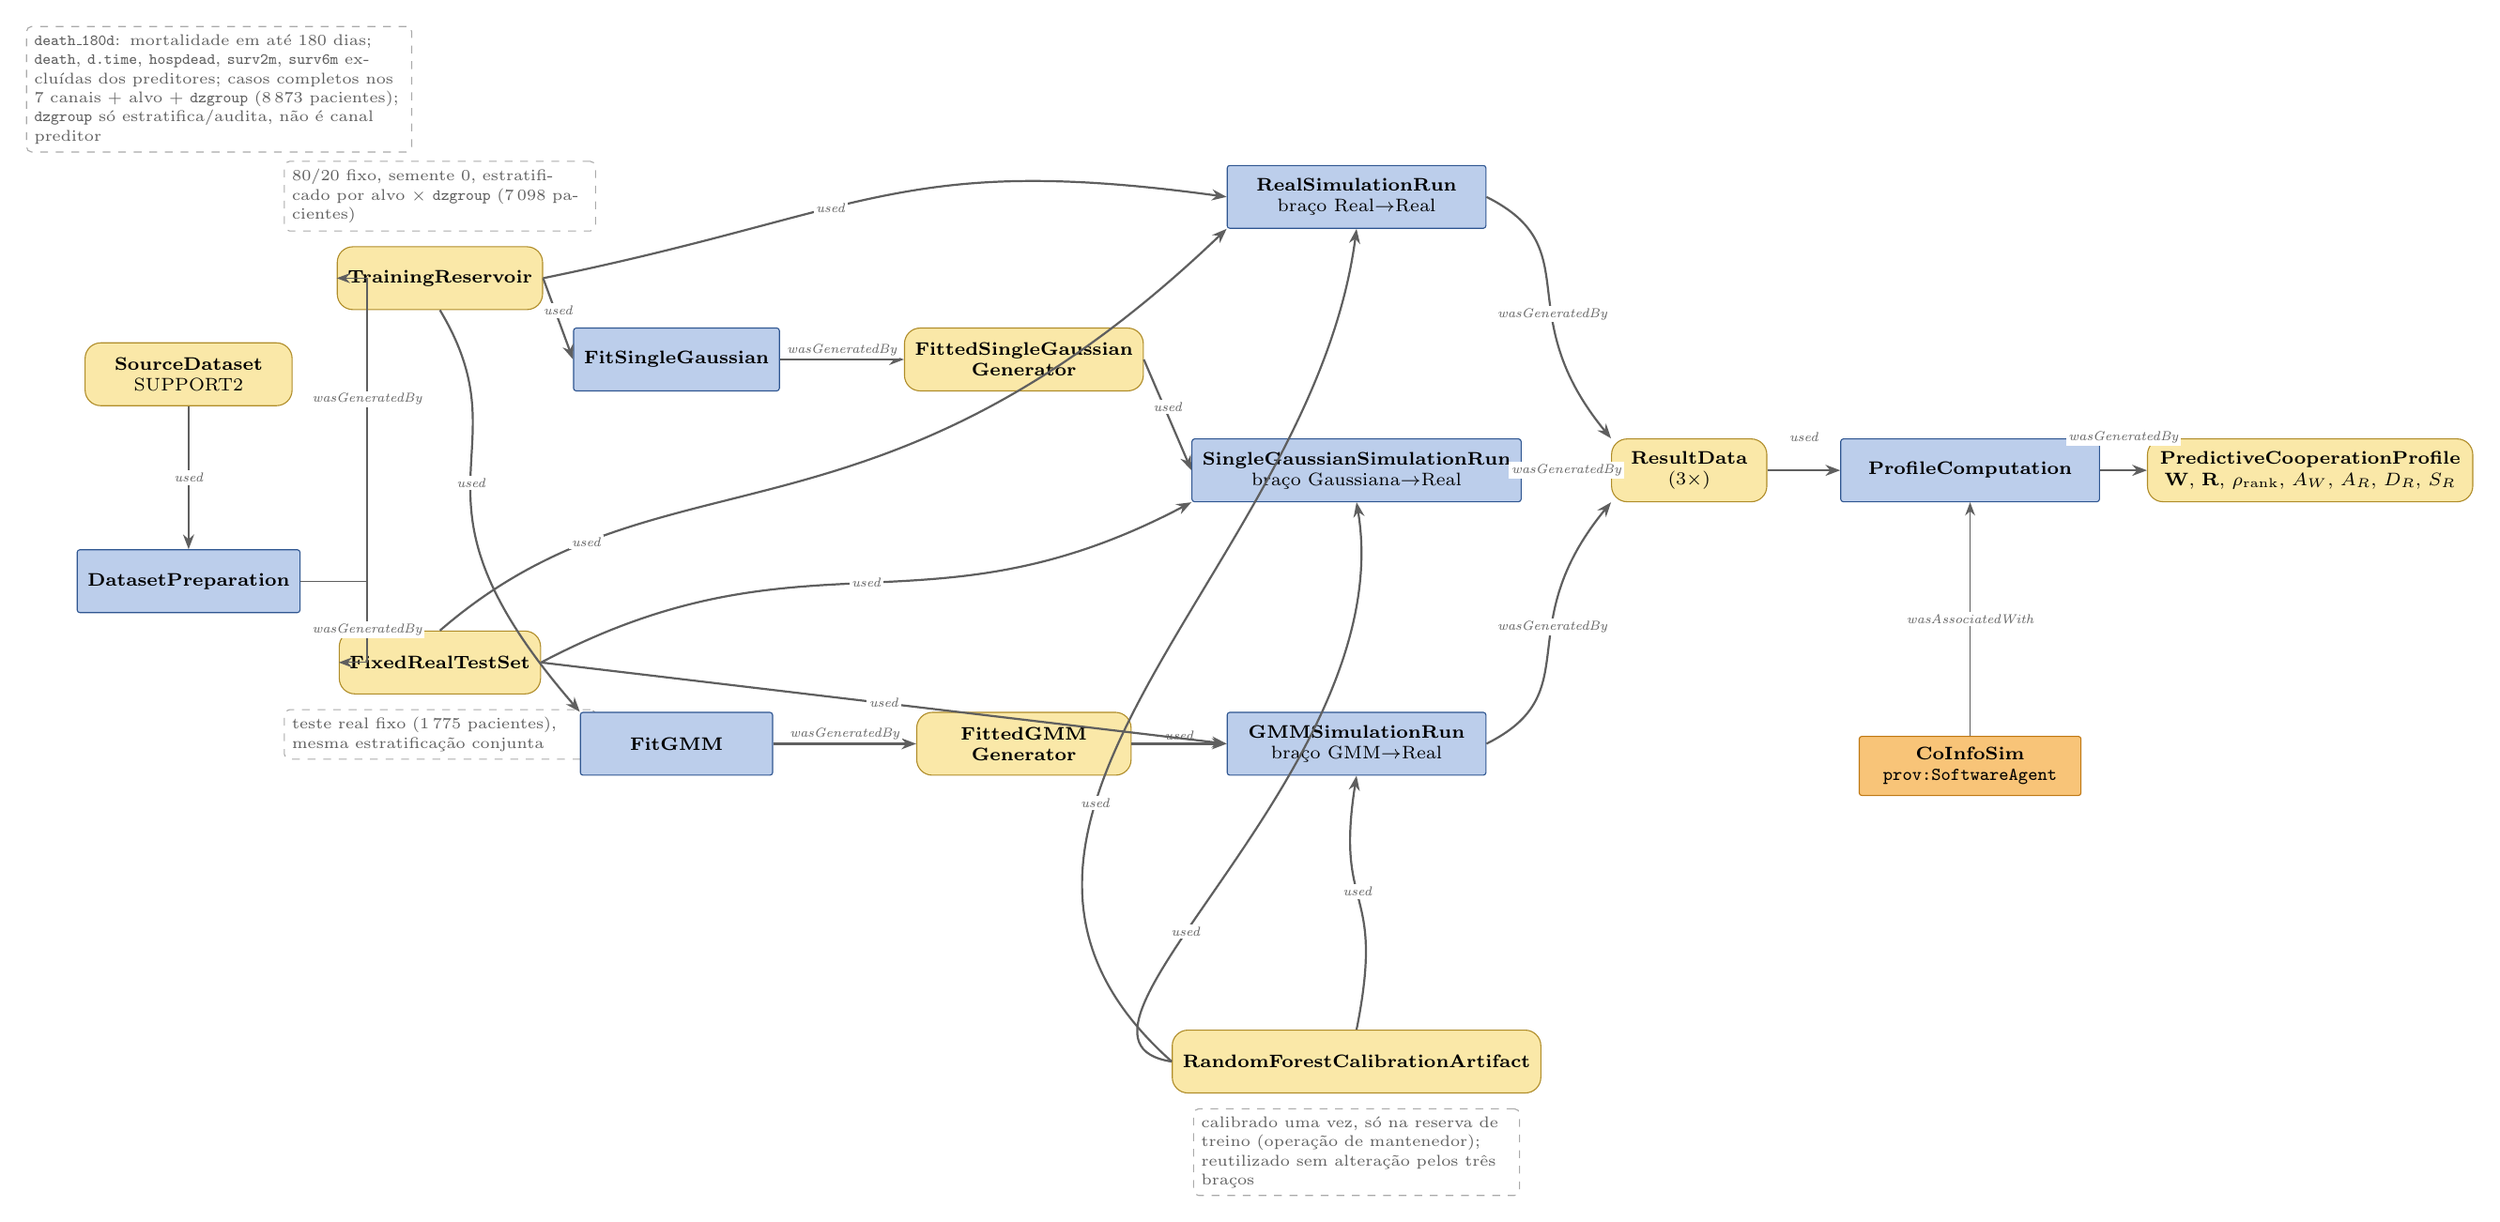
\begin{tikzpicture}[node distance=4mm and 4mm]

  % --- Origem e preparação do dataset -----------------------------------------
  \node[entidade,minimum width=2.8cm]  (source)   at (-3.4, 1.3) {\textbf{SourceDataset}\\SUPPORT2};
  \node[atividade,minimum width=2.8cm] (dataprep) at (-3.4, -1.5) {\textbf{DatasetPreparation}};
  \draw[relacao] (source) -- node[rlabel]{used} (dataprep);

  \node[entidade,minimum width=2.6cm]  (trainres)  at (0, 2.6) {\textbf{TrainingReservoir}};
  \node[entidade,minimum width=2.6cm]  (fixedtest) at (0, -2.6) {\textbf{FixedRealTestSet}};
  \draw[relacaofina] (dataprep.east) -- ++(0.9,0) coordinate (dpbus) |- node[pos=0.3,rlabel]{wasGeneratedBy} (trainres.west);
  \draw[relacaofina] (dpbus) |- node[pos=0.3,rlabel]{wasGeneratedBy} (fixedtest.west);

  \node[nota, text width=4.0cm, above=2mm of trainres] {80/20 fixo, semente 0, estratificado por alvo $\times$ \texttt{dzgroup} (7\,098 pacientes)};
  \node[nota, text width=4.0cm, below=2mm of fixedtest] {teste real fixo (1\,775 pacientes), mesma estratificação conjunta};
  \node[nota, text width=5.0cm, anchor=south west] at (-5.6, 4.3) {\texttt{death\_180d}: mortalidade em até 180 dias; \texttt{death}, \texttt{d.time}, \texttt{hospdead}, \texttt{surv2m}, \texttt{surv6m} excluídas dos preditores; casos completos nos 7 canais + alvo + \texttt{dzgroup} (8\,873 pacientes); \texttt{dzgroup} só estratifica/audita, não é canal preditor};

  \node[atividade,minimum width=2.6cm] (fitgauss) at (3.2, 1.5) {\textbf{FitSingleGaussian}};
  \node[atividade,minimum width=2.6cm] (fitgmm)   at (3.2, -3.7) {\textbf{FitGMM}};

  \node[entidade,minimum width=2.9cm]  (fittedgauss) at (7.9, 1.5)  {\textbf{FittedSingleGaussian}\\\textbf{Generator}};
  \node[entidade,minimum width=2.9cm]  (fittedgmm)   at (7.9, -3.7) {\textbf{FittedGMM}\\\textbf{Generator}};

  \node[atividade,minimum width=3.5cm] (realrun)  at (12.4, 3.7)  {\textbf{RealSimulationRun}\\braço Real$\to$Real};
  \node[atividade,minimum width=3.5cm] (gaussrun) at (12.4, 0)    {\textbf{SingleGaussianSimulationRun}\\braço Gaussiana$\to$Real};
  \node[atividade,minimum width=3.5cm] (gmmrun)   at (12.4, -3.7) {\textbf{GMMSimulationRun}\\braço GMM$\to$Real};

  \node[entidade,minimum width=2.1cm]  (resultdata) at (16.9, 0) {\textbf{ResultData}\\(3$\times$)};
  \node[atividade,minimum width=3.5cm] (profcomp)   at (20.7, 0) {\textbf{ProfileComputation}};
  \node[entidade,minimum width=4.4cm]  (profile)    at (25.3, 0) {\textbf{PredictiveCooperationProfile}\\$\mathbf{W}$, $\mathbf{R}$, $\rho_{\mathrm{rank}}$, $A_W$, $A_R$, $D_R$, $S_R$};

  \draw[relacao] (trainres.east) -- node[rlabel,above]{used} (fitgauss.west);
  \draw[relacao] (trainres.south) .. controls +(1.2,-2.0) and +(-2.6,3.0) .. node[rlabel,pos=0.5]{used} (fitgmm.north west);
  \draw[relacao] (trainres.east) .. controls +(4.4,0.9) and +(-4.4,0.6) .. node[rlabel,pos=0.4]{used} (realrun.west);

  \draw[relacao] (fitgauss.east) -- node[rlabel,above]{wasGeneratedBy} (fittedgauss.west);
  \draw[relacao] (fitgmm.east)   -- node[rlabel,above]{wasGeneratedBy} (fittedgmm.west);
  \draw[relacao] (fittedgauss.east) -- node[rlabel,above]{used} (gaussrun.west);
  \draw[relacao] (fittedgmm.east)   -- node[rlabel,above]{used} (gmmrun.west);

  \draw[relacao] (fixedtest.north) .. controls +(3.0,2.6) and +(-4.8,-4.6) .. node[rlabel,pos=0.22]{used} (realrun.south west);
  \draw[relacao] (fixedtest.east)  .. controls +(3.6,1.9) and +(-3.6,-1.9) .. node[rlabel,pos=0.5]{used} (gaussrun.south west);
  \draw[relacao] (fixedtest.east)  -- node[rlabel]{used} (gmmrun.west);

  % --- Artefato de calibração do Random Forest, compartilhado pelos 3 braços --
  \node[entidade,minimum width=3.2cm] (rfcalib) at (12.4, -8.0) {\textbf{RandomForestCalibrationArtifact}};
  \node[nota, text width=4.2cm, below=2mm of rfcalib] {calibrado uma vez, só na reserva de treino (operação de mantenedor); reutilizado sem alteração pelos três braços};
  \draw[relacao] (rfcalib.north) .. controls +(0.4,2.0) and +(-0.3,-1.9) .. node[rlabel,pos=0.55]{used} (gmmrun.south);
  \draw[relacao] (rfcalib.west)  .. controls +(-2.0,0.3) and +(0.6,-3.6) .. node[rlabel,pos=0.4]{used} (gaussrun.south);
  \draw[relacao] (rfcalib.west)  .. controls +(-3.6,3.2) and +(-0.6,-4.6) .. node[rlabel,pos=0.35]{used} (realrun.south);

  \draw[relacao] (realrun.east)  .. controls +(1.4,-0.7) and +(-1.4,1.7) .. node[rlabel,pos=0.6]{wasGeneratedBy} (resultdata.north west);
  \draw[relacao] (gaussrun.east) -- node[rlabel]{wasGeneratedBy} (resultdata.west);
  \draw[relacao] (gmmrun.east)   .. controls +(1.4,0.7) and +(-1.4,-1.7) .. node[rlabel,pos=0.6]{wasGeneratedBy} (resultdata.south west);

  \draw[relacao] (resultdata) -- node[rlabel,yshift=4.5mm]{used} (profcomp);
  \draw[relacao] (profcomp)   -- node[rlabel,yshift=4.5mm]{wasGeneratedBy} (profile);

  \node[agente] (agent) at (20.7, -4.0) {\textbf{CoInfoSim}\\\texttt{prov:SoftwareAgent}};
  \draw[relacaofina] (agent.north) -- node[rlabel]{wasAssociatedWith} (profcomp.south);

\end{tikzpicture}
\end{document}
